\section{NÚMEROS PRIMOS}
\subsection{Teoría}
\begin{frame}{NÚMEROS PRIMOS}
	\framesubtitle{Teoría}
	\begin{itemize}
      \item Teorema Fundamental de la aritmética
      \item ¿Cuántos primos hay en el intervalo (1,x)?
      \item Teorema de Chebyshev
      \item Problemas clásicos de los primos
	\end{itemize}
    \begin{figure}
    	\centering
        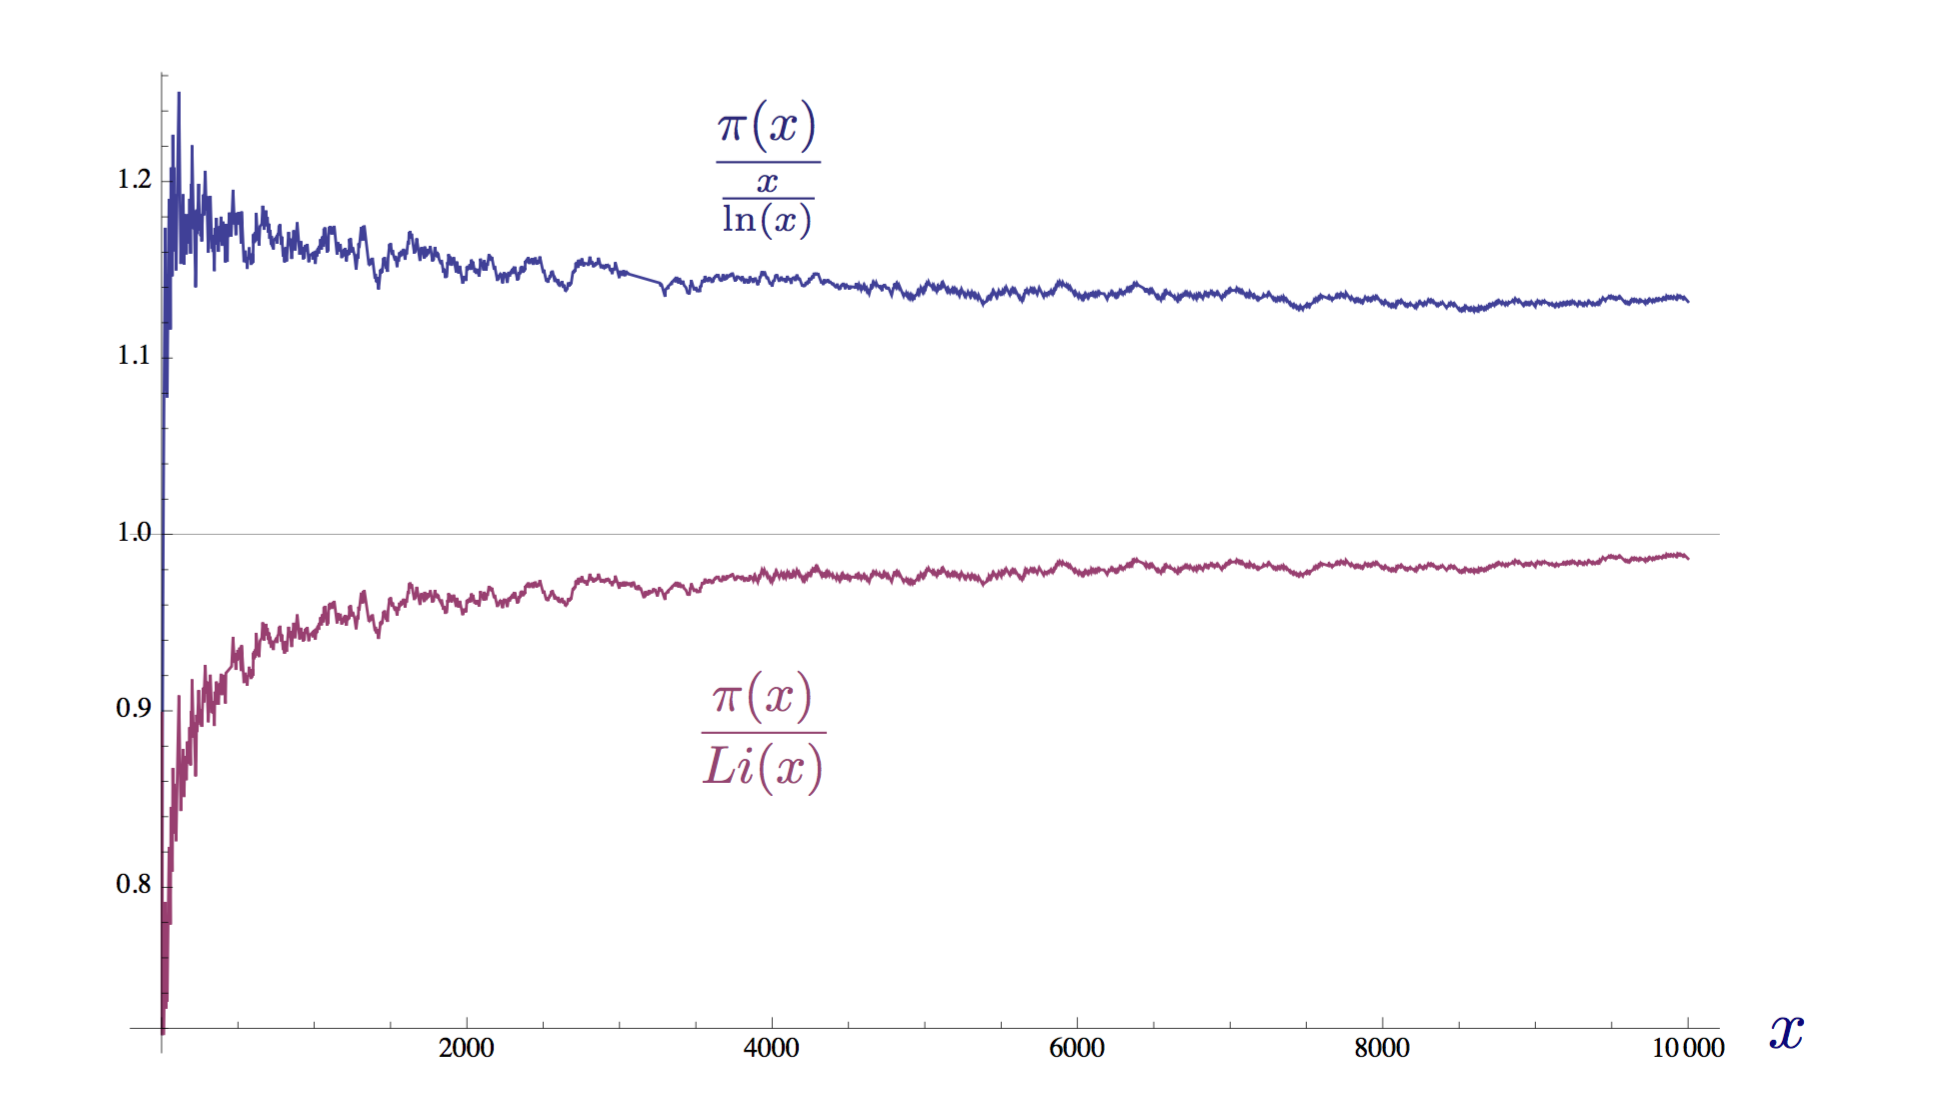
\includegraphics[scale=0.1]{ratioConv.png}
        \caption{Convergencia de la función contadora de primos a 1 por dos aproximaciones\footnotemark{}.}
    \end{figure}
    \vspace{-1cm}\footnotetext{\bibentry{conv}}
\end{frame}
%%%%%%%%%%%%%%%%%%%%%%%%%%%%%%%%%%%%%%%%%%%%%%%%%%%%%%%%%%
\subsection{Adicional}
\begin{frame}{NÚMEROS PRIMOS}
	\framesubtitle{Adicional}
    \begin{itemize}
    \item Función Zeta de Riemann
    	\begin{equation}
    		\zeta (s)=\sum_{n=1}^{\infty}{\frac{1}{n^s}}
    	\end{equation}
    \item Identidad de Euler
    	\begin{equation}
    		\zeta(s)=\prod_{p}{\frac{1}{1-p^{-s}}}
    	\end{equation}
    \end{itemize}
    \begin{figure}
    	\centering
        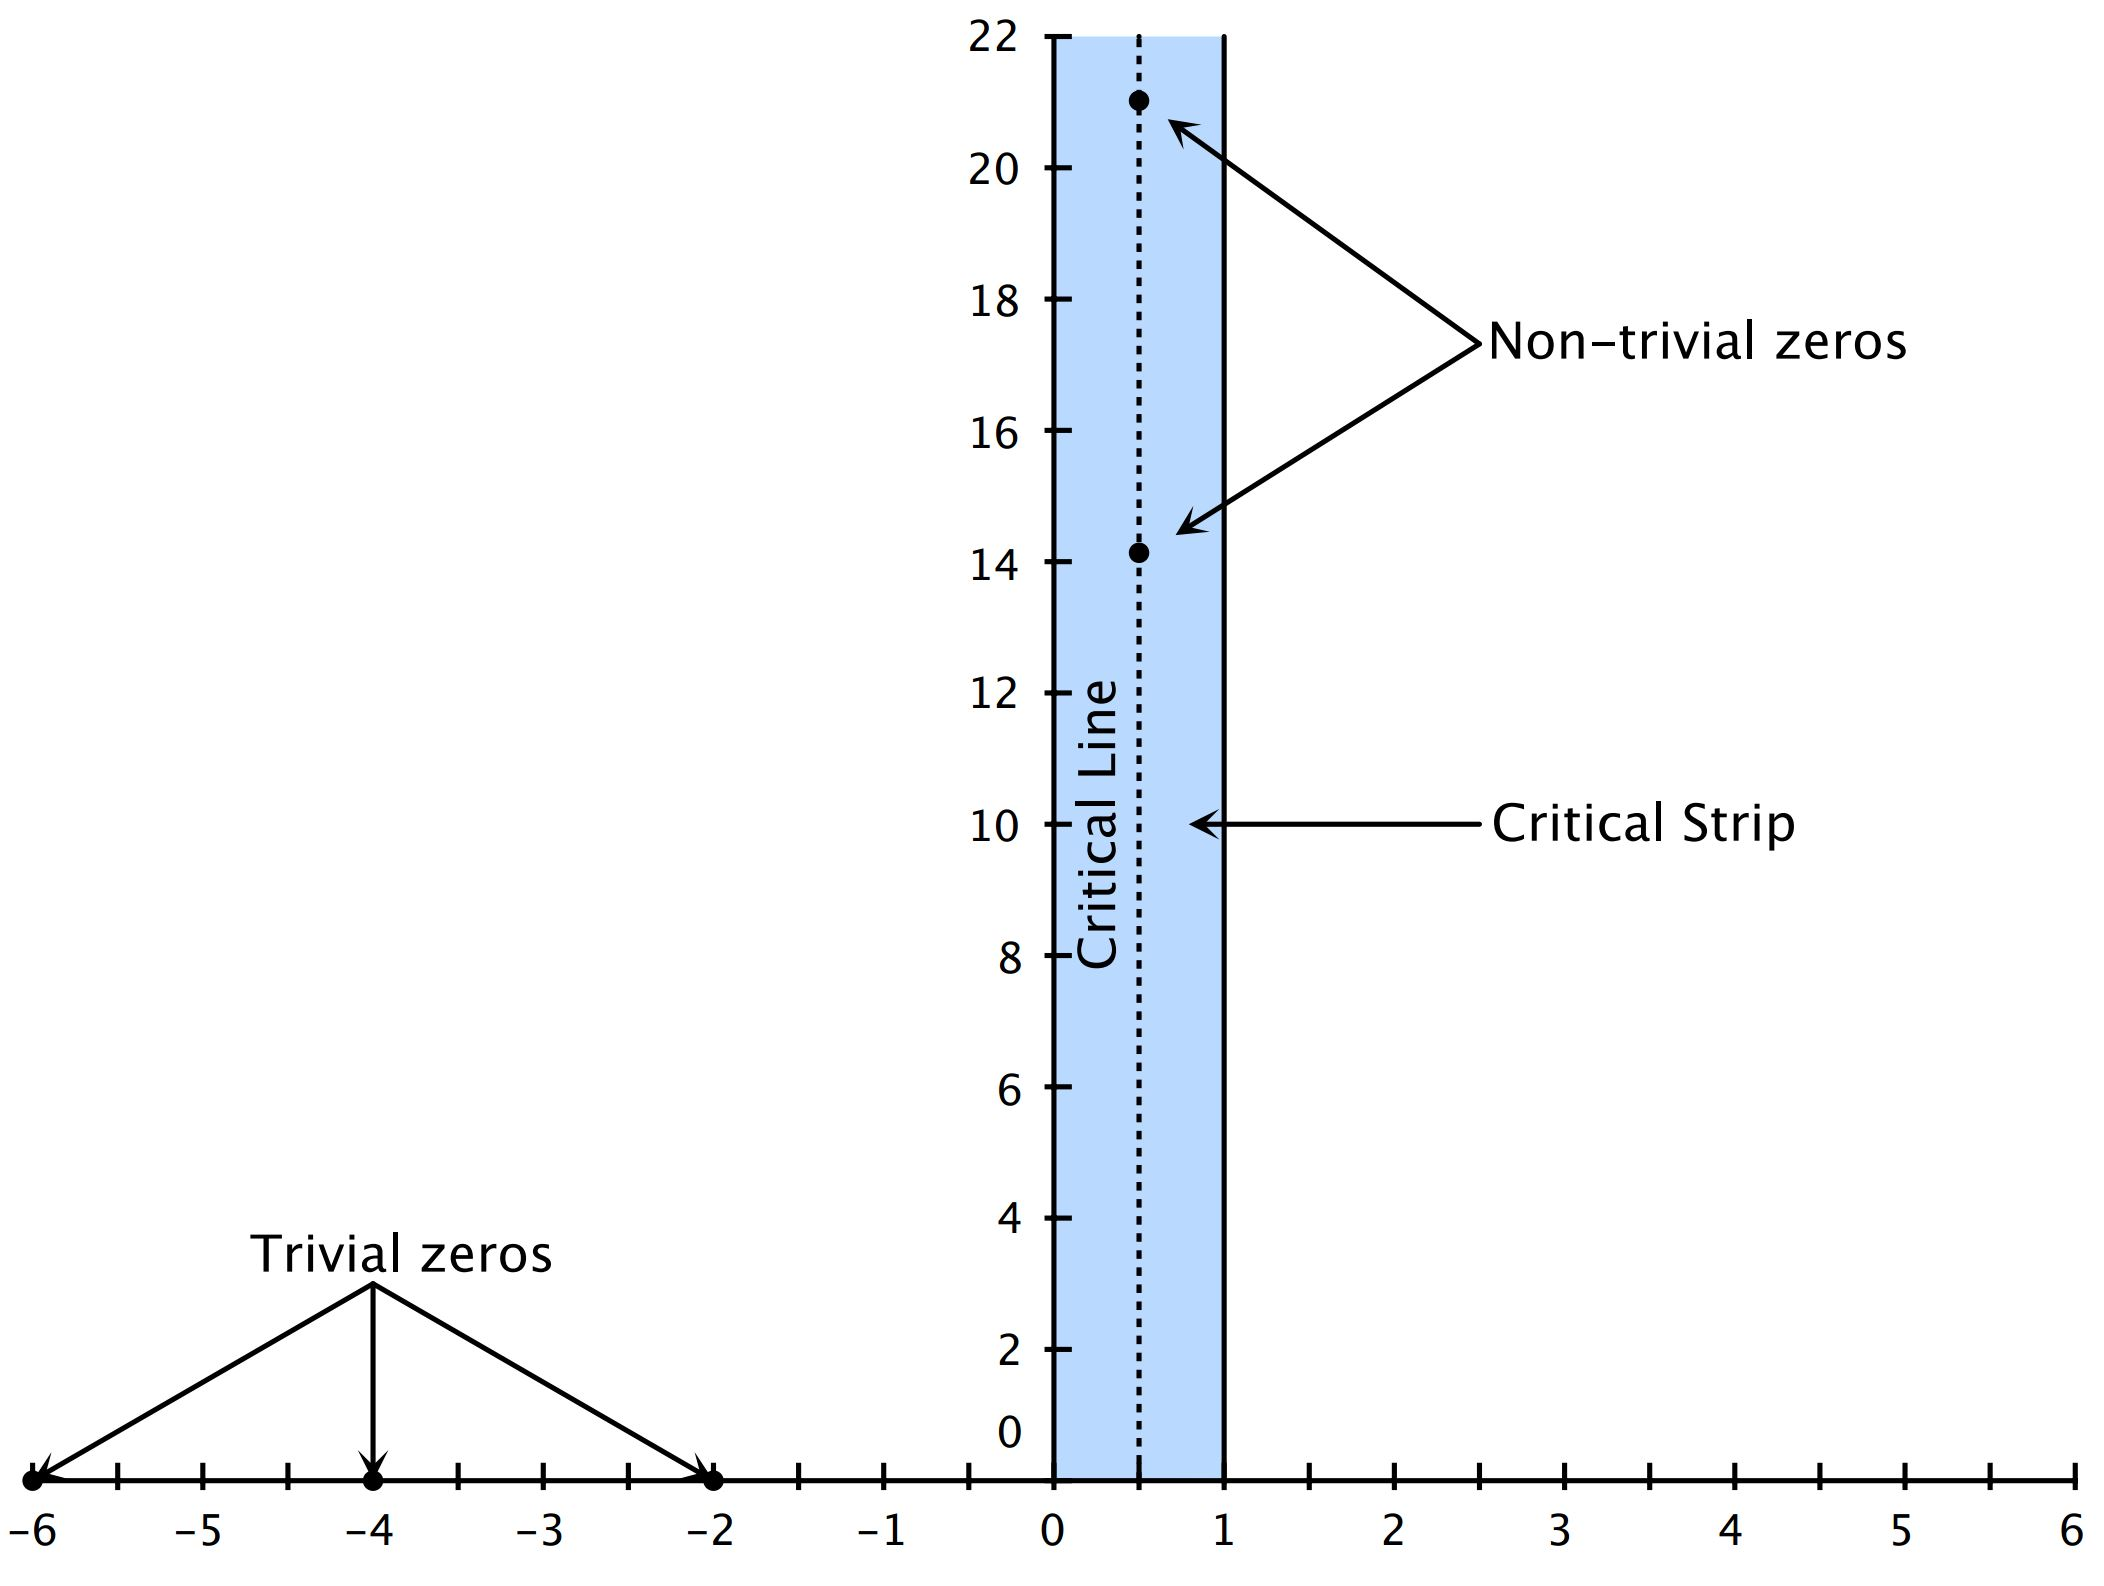
\includegraphics[scale=0.15]{Riemann.JPG}
        \caption{Hipótesis de Riemann\footnotemark{}.}
    \end{figure}
    \vspace{-7mm}\footnotetext{\bibentry{RH}}
\end{frame}
